\begin{center}
    \vspace*{1.5cm}
    {\fontsize{20}{20}\textbf{Rekursiva visor}}\\
    \vspace{0.7cm}
    {\fontsize{12}{12}\textit{Om tålamodet själv får välja}}
\end{center}
\addtocwithheader{Rekursiva visor}  % Add entry to TOC and set header\noBackground
\noBackground

\newpage
\resetBackground

\subsection*{Min gode vän Joel} 
\index[alfa]{Min gode vän Joel}
\index[anfa]{Min gode vän Joel}
\songinfo{Mel: Trampa på gasen}

\begin{parse lines}[\noindent]{#1\\}
    Min gode vän Joel
    Han är en glad kamrat
    Han har äpplen fram och en kulvert bak
    Min gode vän Joel
    Han ser rätt lustig ut
    Man kan kalla honom Knut
    Om man vill
    Och det vill man.
\end{parse lines}

\subsection*{Vår gode vän Jor-el} 
\index[alfa]{Vår gode vän Jor-el}
\index[anfa]{Vår gode vän Jor-el}
\songinfo{Lundakarnevalen 2002}

\begin{parse lines}[\noindent]{#1\\}
    Vår gode vän Jor-El
    Är far till Superman
    Super man som han blir man full som fan
    Min gode vän Jor-El
    Han dricker supersprit
    Men tål inte kryptonit
    Kastar upp i raketen
\end{parse lines}


\newpage

\subsection*{Min Gode Vän Josef} 
\index[alfa]{Min Gode Vän Josef}
\index[anfa]{Min Gode Vän Josef}
\songinfo{Lundakarnevalen 2006}

\begin{parse lines}[\noindent]{#1\\}
    Min gode vän Josef
    Han var på fyllefest
    I tequilarace - han drack allra mest
    Den helige ande
    Slog till och passa på
    Maria kunde inte gå
    På nio månader
\end{parse lines}

\subsection*{Bortom IT-Samhället} 
\index[alfa]{Bortom IT-Samhället}
\index[anfa]{Usama Bin-Ladin}
\songinfo{Lundakarnevalen 2002}

\begin{parse lines}[\noindent]{#1\\}
    Usama Bin-Ladin
    Har ingen SMS
    Ingen ICQ eller mailadress
    Usama Bin-Ladin
    Tycks ha gått upp i rök
    Man kan inte trycka "Sök"
    Om man vill
    Och det vill Bush
\end{parse lines}

\vissteduatt{Visste du att E-sektionen var den sista sektionen på LTH att skapa\\ en egen sångbok?}

\newpage

\subsection*{Jag pluggar på LU} 
\index[alfa]{Jag pluggar på LU}
\index[anfa]{Jag pluggar på LU}
%\songinfo{}

\begin{parse lines}[\noindent]{#1\\}
    Jag pluggar på LU
    Och läser gratispoäng
    När ni gör er labb
    Ligger jag i säng
    Jag pluggar på LU
    Tar inga hårda tag
    Men ändå får jag bidrag
    Från CSN
    Ja, det får jag    
\end{parse lines}

\subsection*{Jag kuggade tentan} 
\index[alfa]{Jag kuggade tentan}
\index[anfa]{Jag kuggade tentan}
%\songinfo{}

\begin{parse lines}[\noindent]{#1\\}
    Jag kuggade tentan
    Men det gör inte nått
    För jag hade ändå inga pengar fått
    För om man blir ratad
    Av hela CSN
    Får man ofta ringa hem
    För att få lite pengar    
\end{parse lines}


\newpage

\begin{textblock*}{3cm}(4.4cm,8.3cm) % {width}(x, y)
    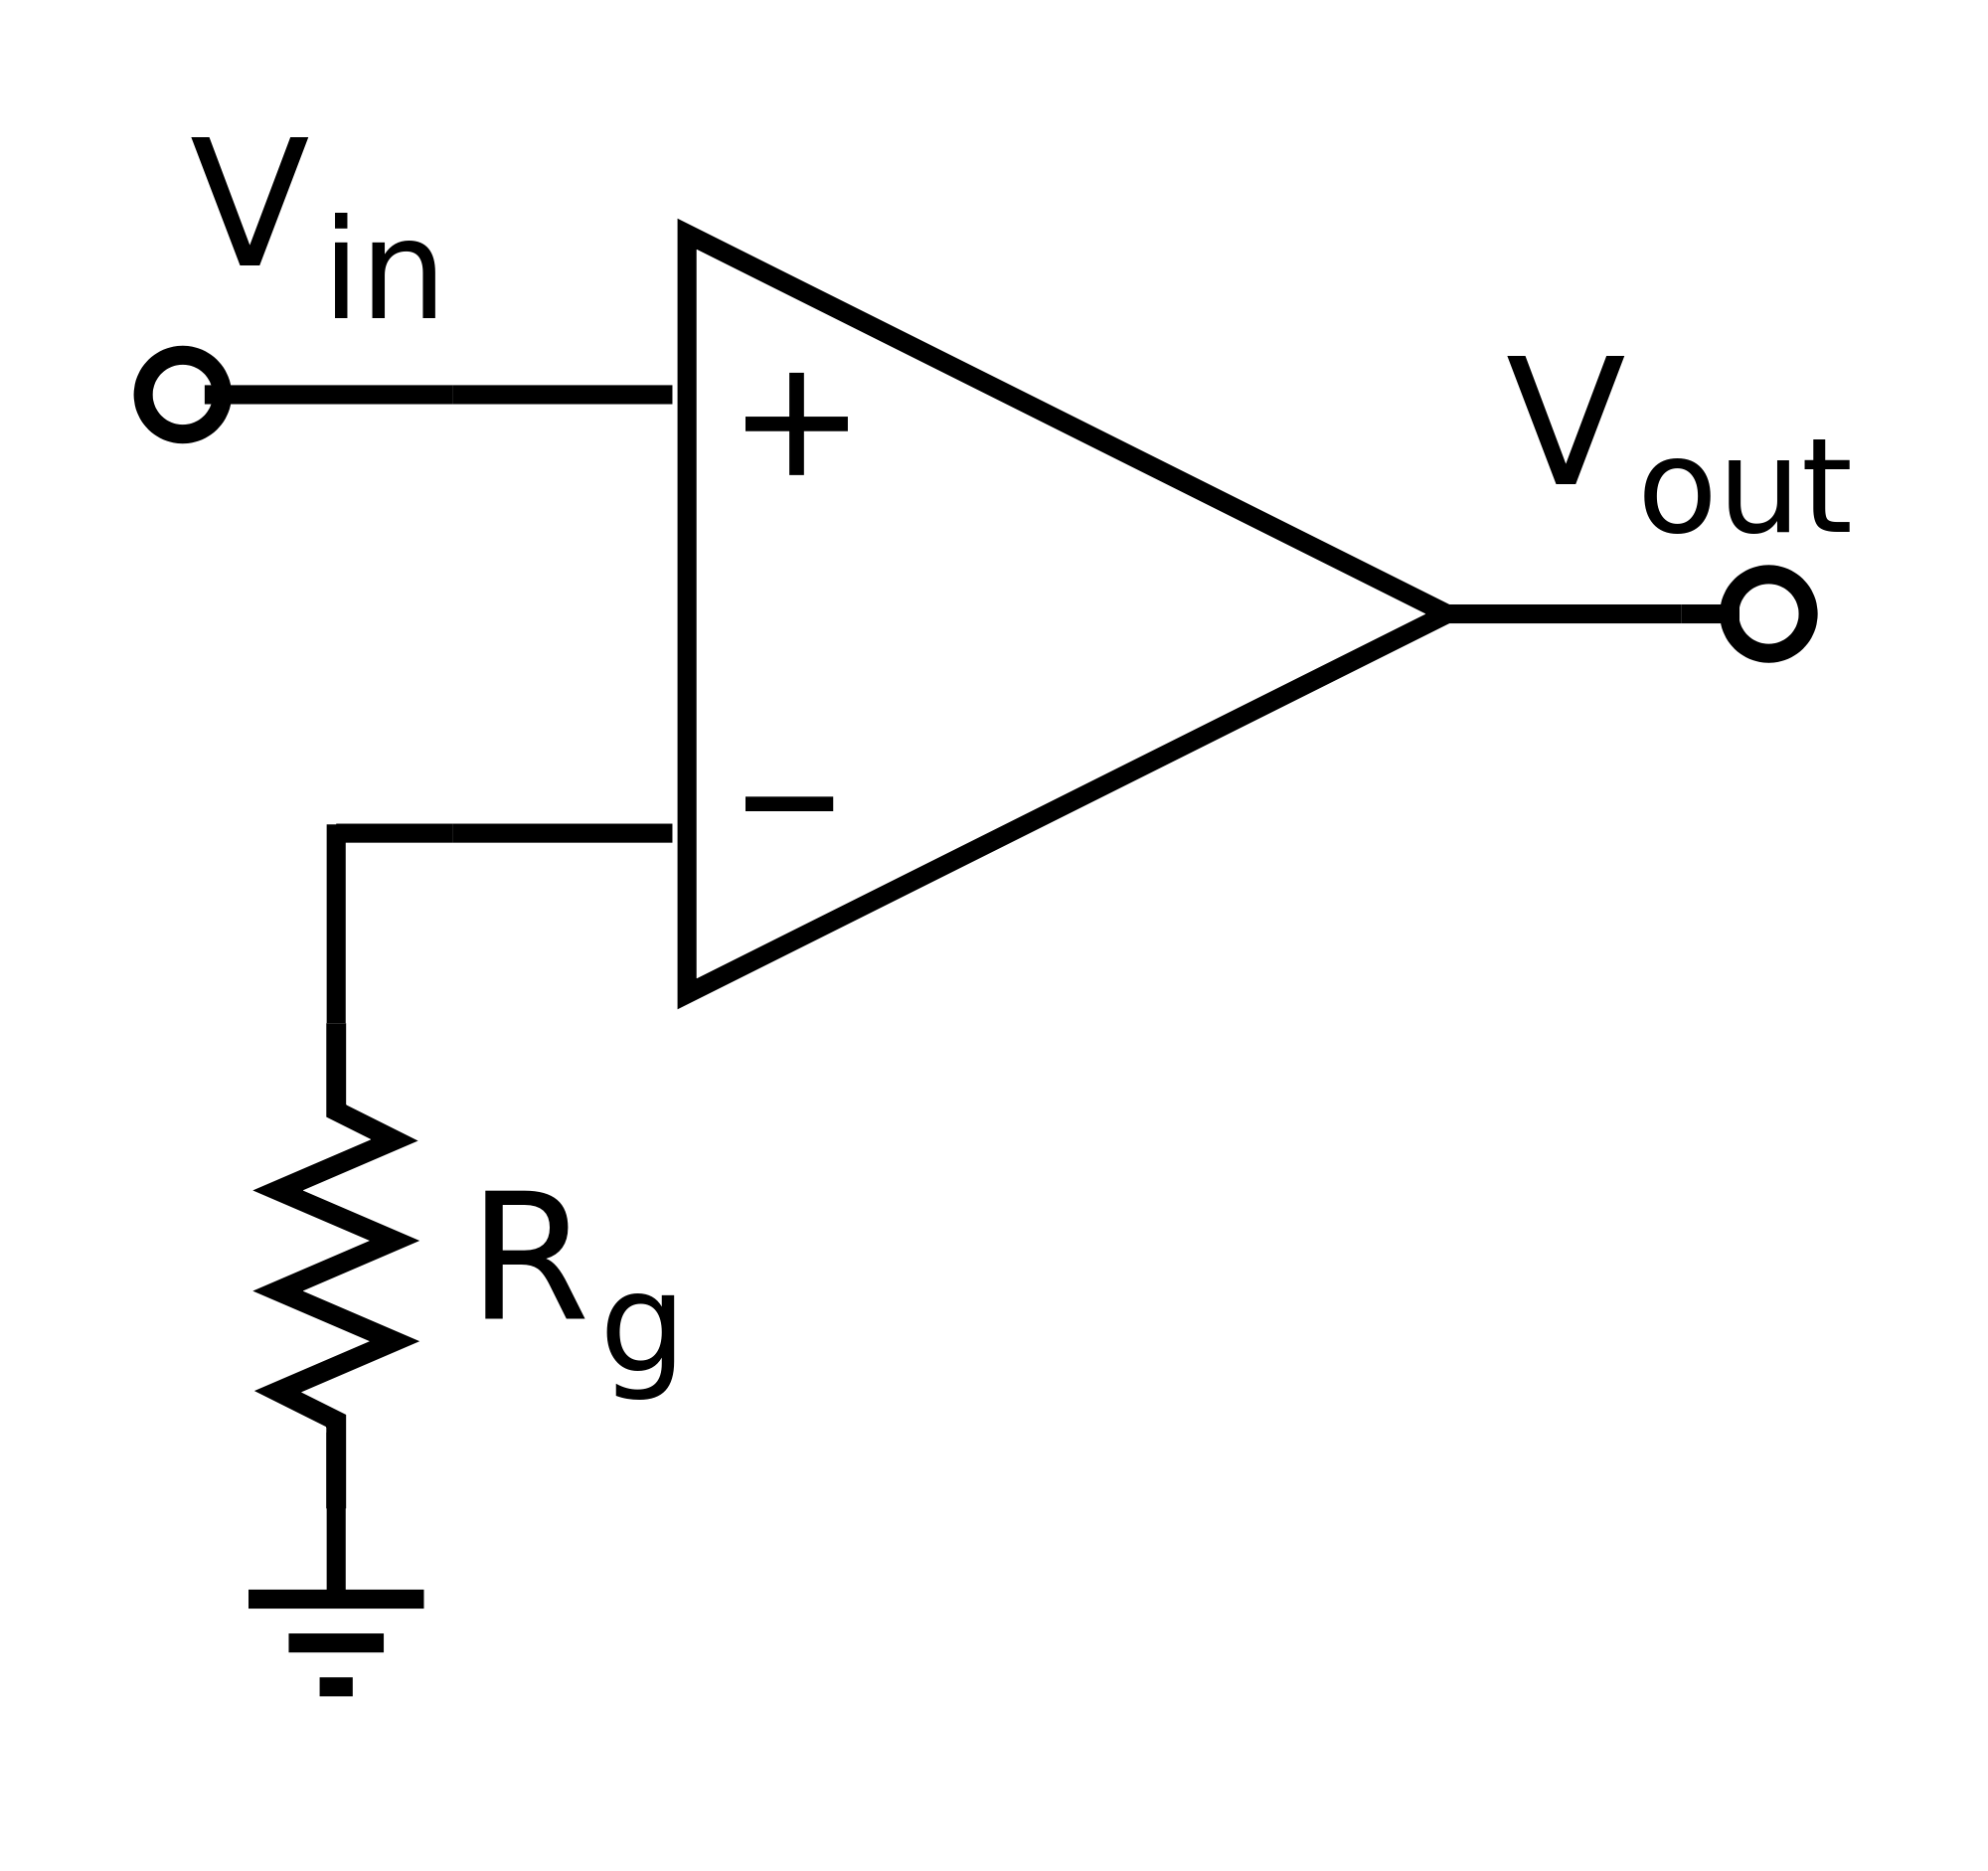
\includegraphics[width=5.6cm]{./bilder/OP-förstärkare.png}
\end{textblock*}


\subsection*{Jag drikker Tuborg} 
\index[alfa]{Jag drikker Tuborg}
\index[anfa]{Jag drikker Tuborg}
\songinfo{Mel: Trampa på gasen\\
synge på dansk}

\begin{parse lines}[\noindent]{#1\\}
    Jeg drikker Tuborg
    og snapser gammeldansk
    Det ær alt jeg vil,
    det ær alt jeg kan
    Jeg drikker Tuborg
    og snapser gammeldansk
    Det ær alt jeg vil og kan,
    så hold kæft jeg ær lykkelig!
\end{parse lines}

\subsection*{Alla är söta} 
\index[alfa]{Alla är söta}
\index[anfa]{Alla på eko}
%\songinfo{}

\begin{parse lines}[\noindent]{#1\\}
    Alla på eko
    Har koll på vårt klimat
    Utan dom får vi förgiftad mat
    Och dom på Eko
    Älskar alla djur
    Och det tycker vi är tur
    För dom är så söta   
\end{parse lines}

\vissteduatt{Visste du att E-sektionen var den sista sektionen på LTH som\\skapade en egen sångok?}

\newpage

\subsection*{Måsen} 
\index[alfa]{Måsen}
\index[anfa]{Det satt en mås}
\songinfo{Mel: När månen vandrar}

\begin{parse lines}[\noindent]{#1\\}
    Det satt en mås på en klyvarbom
    Och tom i krävan var kräket
    Och tungan lådde i skeppar'ns gom
    Där han satt uti bleket
    Jag vill ha sill hördes måsen rope
    Och skeppar'n svarte: Jag vill ha OP
    Om blott jag får, om blott jag får
    
    Nu lyfter måsen från klyvarbom
    Och vinden spelar i tågen
    OP:n svalkat har skeppar'ns gom
    Jag önskar blott att jag såg 'en
    Så nöjd och lycklig, den arme saten
    Han sätter storsegel den krabaten
    Till sjöss han far, och halvan tar
    
    Den mås som satt på en klyvarbom
    Den är nu död och begraven
    Och skeppar'n som drack en flaska rom
    Han har nu drunknat i haven
    Så kan det gå om man fått för mycké
    Om man för brännvin har fattat tycke
    Vi som har kvar, vi resten tar
    
\end{parse lines}

\newpage

\subsection*{Musen} 
\index[alfa]{Musen}
\index[anfa]{Det satt en mus}
%\songinfo{}

\begin{parse lines}[\noindent]{#1\\}
    Det satt en mus i en hushållsost
    Och åt och åt utan måtta
    Tills osten blivit en mushåls-ost
    Och han en klotformad råtta
    "Så bra", sa musen, "att va en fettboll,
    Nu kan jag rulla med hast åt rätt håll:
    Ostindien! Ostindien!"
\end{parse lines}

\subsection*{Moosen} 
\index[alfa]{Moosen}
\index[anfa]{Det satt en älg}
%\songinfo{}
\begin{parse lines}[\noindent]{#1\\}
    Det satt en älg i en klyvartopp
    Förklädd i älgjaktens månad
    Han var befjädrad till horn och kropp
    Och skepparn blev smått förvånad
    "Jag är en mås, goa skepparn" ljög den
    Förklädda älgen, därefter flög den
    Mjukt föll han sen
    På skepparen
\end{parse lines}

\subsection*{Mesen} 
\index[alfa]{Mesen}
\index[anfa]{Det satt en mes}
%\songinfo{}

\begin{parse lines}[\noindent]{#1\\}
    Det satt en mes i en klyvarmast
    Där sågs han ragla och svaja
    För trots att frön var hans enda last
    Var han full som en kaja
    "Vad har du gjort!" hördes skepparn stöna
    Och mesen svarte "Jag rökte fröna
    I egen holk, i egen holk."
\end{parse lines}

\newpage

\subsection*{Boten} 
\index[alfa]{Boten}
\index[anfa]{Min kompis Anna}
%\songinfo{}

\begin{parse lines}[\noindent]{#1\\}
    Min kompis Anna, hon är en bot
    Hon rensar upp i kanalen
    Och varje gång jag hör hennes låt
    Så får jag ont i analen
    Jag är så trött på den jävla låten
    Kan någon vänlig själ banna boten?
    Jag vete fan
    Jag fick en ban
\end{parse lines}

\subsection*{Kompistipset} 
\index[alfa]{Kompistipset}
\index[anfa]{Min kompis Bosse}
%\songinfo{}

\begin{parse lines}[\noindent]{#1\\}
    Min kompis Bosse, en bigamist
    Tar alltid två öl i baren
    Han säger "Allting kan verka trist
    Ifall man blott bara tar en
    Nej, ta och skaffa dig en till fru å
    Be alltid bartendern om en duo
    Så skål min vän, och skål igen!"
\end{parse lines}

\subsection*{När månen vandrar} 
\index[alfa]{När månen vandrar}
\index[anfa]{När månen vandrar}
%\songinfo{}

\begin{parse lines}[\noindent]{#1\\}
    När månen vandrar sin tysta ban
    Och tittar in genom rutan
    Då tänker jag, att på ljusan da'n
    Då kan jag klara mig utan
    Då kan jag klara mig utan måne
    Men utan Renat och utan Skåne?
    Det vete fan, det vete fan    
\end{parse lines}

\newpage

\subsection*{När måsen vandrar} 
\index[alfa]{När måsen vandrar}
\index[anfa]{Om du en sittning}
%\songinfo{}

\begin{parse lines}[\noindent]{#1\\}
    Om du en sittning vill sakta ner 
    och alla gästerna störa 
    Ja då räcker det att de ser 
    att de nu måsen ska köra 
    Den jävla låten, den är så tråkig 
    “Men den här texten är inte pjåkig” 
    Den åker ut 
    Så håll din trut
\end{parse lines}

\subsection*{JAS:en} 
\index[alfa]{JAS:en}
\index[anfa]{Där flög en JAS över Västerbron}
%\songinfo{}

\begin{parse lines}[\noindent]{#1\\}
    Där flög en JAS över Västerbron
    Men styrsystemet var trasigt
    Piloten sköt ut sig med kanon
    För planet svängde så knasigt
    "Jag vill ju uppåt, jag vill ju mer"
    Men planet svarte: "Jag vill ju ner
    Mot alla hjon, på Västerbron" 
\end{parse lines}


\begin{textblock*}{10cm}(0.0cm, 0.5cm) % {width}(x, y)
    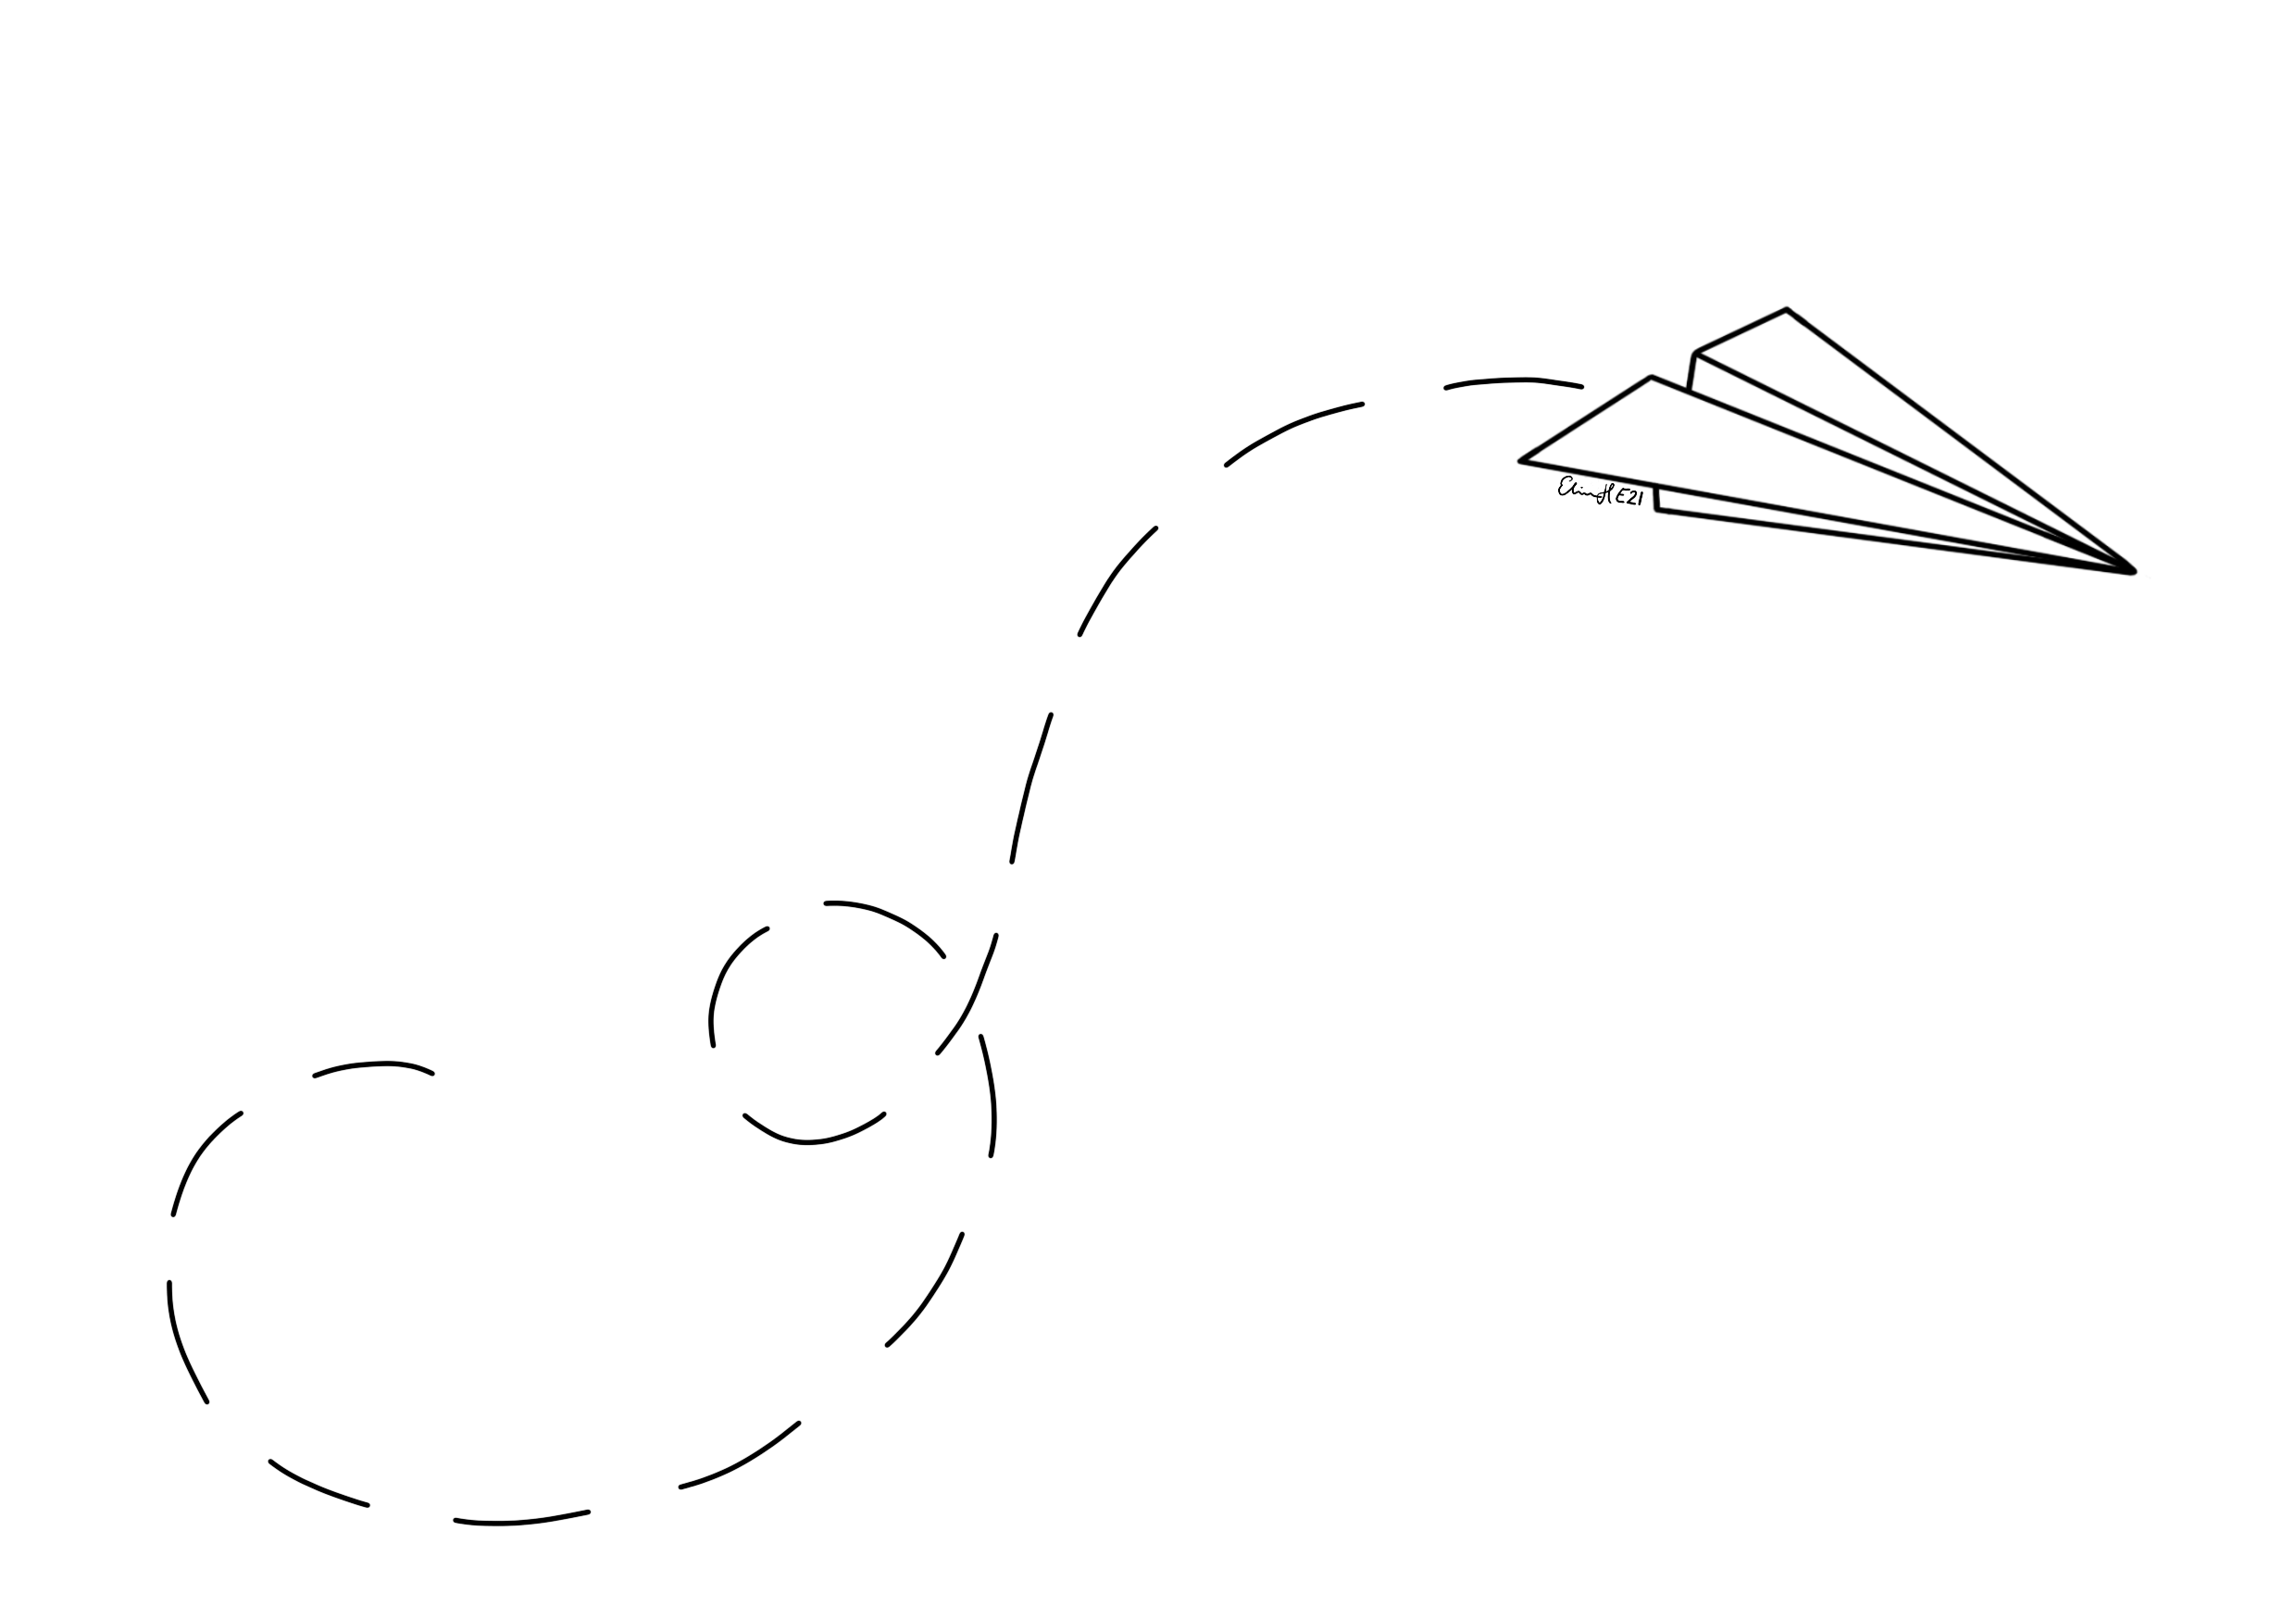
\includegraphics[width=20cm]{./bilder/pappersplan_signerad.png}
\end{textblock*}

\newpage
\noBackground

\begin{comment}
\begin{textblock*}{10cm}(1.0cm, 1.0cm) % {width}(x, y)
    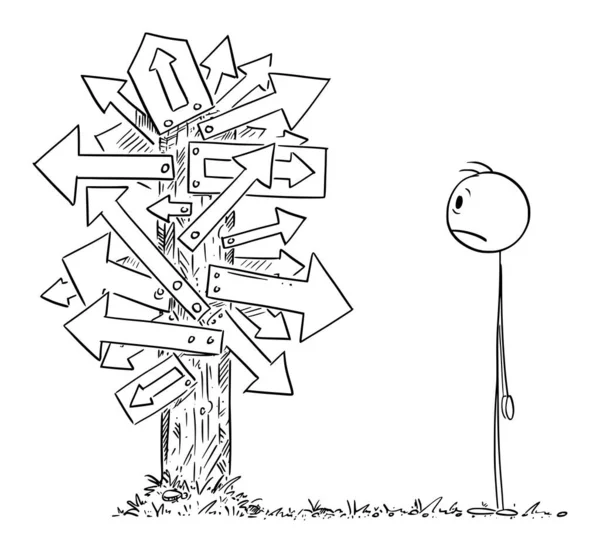
\includegraphics[width=20cm]{./bilder/roda_havet_test.png}
\end{textblock*}

\vspace*{5cm}
\end{comment}

\begin{textblock*}{10cm}(-10.3cm, 0.3cm) % {width}(x, y)
    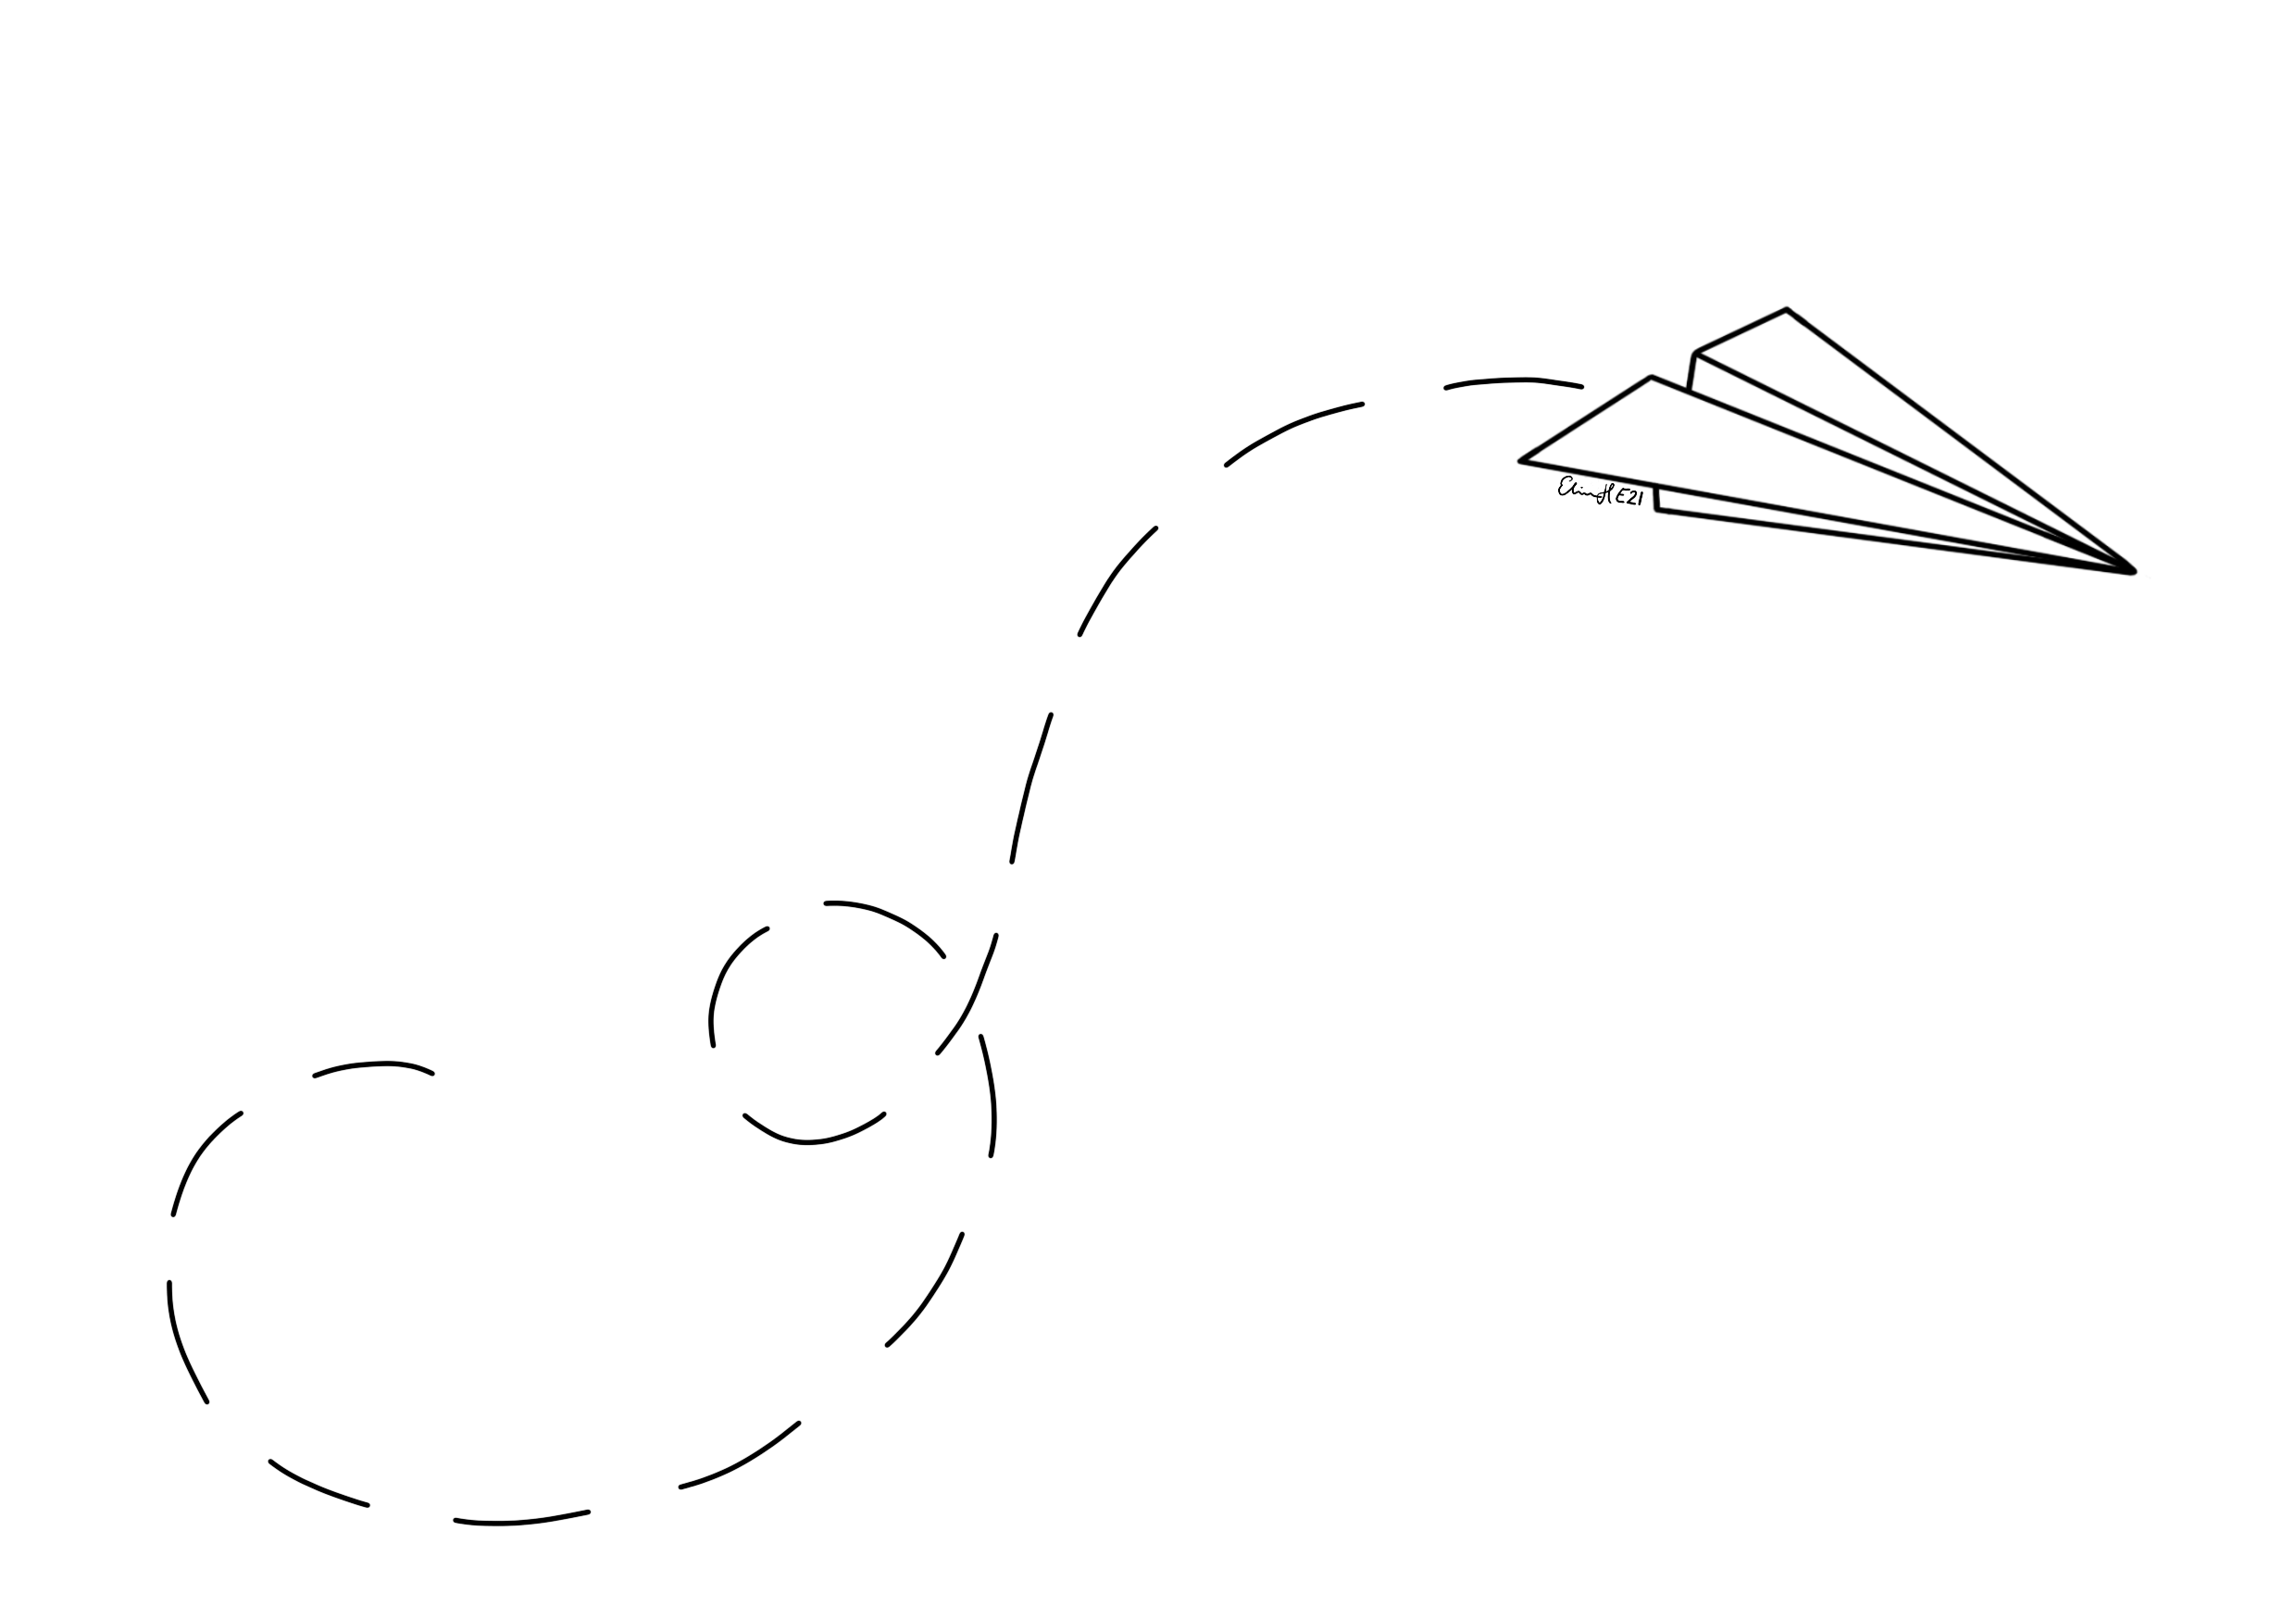
\includegraphics[width=20cm]{./bilder/pappersplan_signerad.png}
\end{textblock*}

\vspace*{5cm}
\subsection*{Röda havet} 
\index[alfa]{Röda havet}
\index[anfa]{Vi gingo ner till Röda havet}
\songinfo{Mel: Skrattvisa ur Orfeus i underjorden, "Pour séduire Alcmène a la fière"}

\begin{parse lines}[\noindent]{#1\\}
    Vi gingo ned till Röda havet
    Vi lågo i där minst en kvart
    Ja, minst en kvart
    Men inte blev vi röda av 'et
    Men Röda havet det blev svart
    
    Men utav aqvavit
    Människan till kropp och själ
    Blir oskuldsfull och vit
    Men utav aqvavit
    Människan till kropp och själ
    Blir oskuldsfull och vit
\end{parse lines}

\newpage
\resetBackground

\subsection*{Stadsparksdammen} 
\index[alfa]{stadsparksdammen}
\index[anfa]{Vi gingo ner till stadsparksdammen}
%\songinfo{}

\begin{parse lines}[\noindent]{#1\\}
    Vi gingo ner till stadsparksdammen
    Vi lågo i där minst en kvart
    Ja, minst en kvart
    Men inte blev vi av med skammen
    Men stadsparksdammen den blev svart
    
    Men utav aqvavit…

\end{parse lines}

\subsection*{Lommabukten} 
\index[alfa]{Lommabukten}
\index[anfa]{Vi gingo ned till Lommabukten}
%\songinfo{}

\begin{parse lines}[\noindent]{#1\\}
    Vi gingo ned till Lommabukten
    Vi lågo i där minst en kvart
    Ja, minst en kvart.
    Men inte blev vi av med lukten
    Men Lommabukten den blev svart
    
    Men utav aqvavit...
\end{parse lines}

\newpage

\subsection*{Finska viken} 
\index[alfa]{Finska viken}
\index[anfa]{Vi gingo ner till Finska viken}
%\songinfo{}

\begin{parse lines}[\noindent]{#1\\}
    Vi gingo ner till Finska viken
    Vi lågo i där minst en kvart
    Ja, minst en kvart
    Men inte blev vi av med skiten
    men Finska viken den blev svart
    
    Men utav aqvavit…

\end{parse lines}

\subsection*{Systembolaget} 
\index[alfa]{Systembolaget}
\index[anfa]{Vi gingo ner till Systembolaget}
%\songinfo{}

\begin{parse lines}[\noindent]{#1\\}
    Vi gingo ner till Systembolaget
    Vi stod i kö där minst en kvart
    Ja, minst en kvart
    Men inte blev vi fulla av det
    Systembolaget det gick back
    
    Men utav aqvavit…
\end{parse lines}

\vissteduatt{Visste du att Aqvavit = aqua vite = livets vatten?}
\newpage

\subsection*{Lablokalen} 
\index[alfa]{Lablokalen}
\index[anfa]{Vi gingo ned till lablokalen}
%\songinfo{}

\begin{parse lines}[\noindent]{#1\\}
    Vi gingo ned till lablokalen
    Vi var där inne minst en kvart
    Ja, minst en kvart.
    Men inte blev vi av med kvalen
    Men lablokalen den blev svart
    
    Men utav aqvavit...
\end{parse lines}

\subsection*{Vi gingo ner till Edekvata} 
\index[alfa]{Vi gingo ner till Edekvata}
\index[anfa]{Vi gingo ner till Edekvata}
%\songinfo{}

\begin{parse lines}[\noindent]{#1\\}
    Vi gingo ner till Edekvata
    Vi olja borden minst en kvart
    Ja, minst en kvart
    Men manualen den vi rata
    så Edekvata det blev svart
    
    Men utav aqvavit…
    
\end{parse lines}

\vissteduatt{Visste du att det brann i Edekvata 2010?
\\En trasa med linolja självantände...}
\newpage

\subsection*{Karnevalen} 
\index[alfa]{Karnevalen}
\index[anfa]{Vi gingo ner till karnevalen}
%\songinfo{}

\begin{parse lines}[\noindent]{#1\\}
    Vi gingo ner till karnevalen
    Och stod i kö där minst en kvart
    Ja, minst en kvart
    Vi ville in i AF-salen
    Men inte fan kom vi nå'n vart

    För utav kösystem
    Blir det bara skit och massa allmänna problem
    För utav kösystem
    Blir det bara skit och massa allmänna problem
    
    Och vi kom fram till kravallstaketet
    Och stod kvar där minst en kvart
    Ja, minst en kvart
    Sen vi var fast i köhelvetet
    Så inte fan kom vi nå'n vart
    
    För utav kösystem…
    
\end{parse lines}


\newpage

tom sida

\newpage